% Cryptographic Hash Functions Analysis Template
% Topics: SHA-256, collision resistance, avalanche effect, birthday attacks
% Style: Cryptographic analysis with computational demonstrations

\documentclass[a4paper, 11pt]{article}
\usepackage[utf8]{inputenc}
\usepackage[T1]{fontenc}
\usepackage{amsmath, amssymb}
\usepackage{graphicx}
\usepackage{siunitx}
\usepackage{booktabs}
\usepackage{subcaption}
\usepackage[makestderr]{pythontex}
\usepackage{algorithm}
\usepackage{algpseudocode}

% Theorem environments
\newtheorem{definition}{Definition}[section]
\newtheorem{theorem}{Theorem}[section]
\newtheorem{property}{Property}[section]
\newtheorem{example}{Example}[section]

% Hyperref must be loaded last
\usepackage[hidelinks]{hyperref}

\title{Cryptographic Hash Functions: SHA-256 Analysis and Security Properties}
\author{Cryptography Research Laboratory}
\date{\today}

\begin{document}
\maketitle

\begin{abstract}
This report presents a comprehensive computational analysis of cryptographic hash functions,
with focus on the SHA-256 algorithm and its security properties. We examine the three
fundamental requirements of cryptographic hash functions: preimage resistance, second preimage
resistance, and collision resistance. Through computational experiments, we demonstrate the
avalanche effect where single-bit input changes produce dramatically different hash outputs,
analyze birthday attack probabilities for collision finding, and explore applications in
digital signatures, blockchain technology, and password hashing. Results confirm SHA-256's
strong security properties including 50\% bit flip probability under minimal input perturbation.
\end{abstract}

\section{Introduction}

Cryptographic hash functions serve as fundamental building blocks in modern information security,
providing data integrity verification, digital signature schemes, and secure password storage.
A cryptographic hash function transforms arbitrary-length input messages into fixed-length
digest values, designed to make finding two inputs with identical outputs computationally infeasible.

\begin{definition}[Cryptographic Hash Function]
A cryptographic hash function $H: \{0,1\}^* \rightarrow \{0,1\}^n$ maps arbitrary-length
bit strings to fixed-length $n$-bit outputs (digests), satisfying three security properties:
\begin{enumerate}
\item \textbf{Preimage resistance}: Given hash value $h$, computationally infeasible to find $m$ such that $H(m) = h$
\item \textbf{Second preimage resistance}: Given $m_1$, infeasible to find $m_2 \neq m_1$ with $H(m_1) = H(m_2)$
\item \textbf{Collision resistance}: Infeasible to find any pair $(m_1, m_2)$ with $m_1 \neq m_2$ and $H(m_1) = H(m_2)$
\end{enumerate}
\end{definition}

\section{Theoretical Framework}

\subsection{SHA-256 Construction}

The Secure Hash Algorithm 256-bit (SHA-256) employs the Merkle-Damg\r{a}rd construction,
processing the input message in 512-bit blocks through iterative compression. The algorithm
initializes eight 32-bit working variables with predetermined constants, then updates these
values through 64 rounds of bitwise operations including rotations, XOR, AND, and modular addition.

\begin{theorem}[Merkle-Damg\r{a}rd Construction]
Let $f: \{0,1\}^{n+m} \rightarrow \{0,1\}^n$ be a collision-resistant compression function.
The iterated hash function $H$ constructed by padding the input, partitioning into $m$-bit
blocks, and iteratively applying $f$ is also collision-resistant. A collision in $H$ implies
a collision in $f$.
\end{theorem}

\subsection{Avalanche Effect}

\begin{property}[Strict Avalanche Criterion]
A cryptographic hash function exhibits the avalanche effect if changing a single input bit
causes each output bit to flip with probability $\approx 0.5$. For an ideal $n$-bit hash
function, a one-bit input change should produce an expected Hamming distance of $n/2$ bits
in the output.
\end{property}

The avalanche effect ensures that similar messages produce dramatically different hash values,
preventing attackers from deducing relationships between inputs based on hash similarity.
SHA-256's compression function achieves excellent avalanche propagation through its round
structure combining non-linear Boolean functions with bit rotations.

\subsection{Birthday Attack Complexity}

\begin{theorem}[Birthday Bound]
For a hash function outputting $n$-bit digests, the expected number of random hash evaluations
required to find a collision is approximately $\sqrt{2^n} = 2^{n/2}$. This follows from the
birthday paradox: among $k$ randomly selected values from a set of size $N$, the collision
probability approaches 0.5 when $k \approx 1.177\sqrt{N}$.
\end{theorem}

For SHA-256 with 256-bit output, birthday attacks require approximately $2^{128}$ hash
evaluations to find a collision with 50\% probability—a computationally infeasible number
even for state-of-the-art computing clusters.

\begin{example}[Birthday Paradox]
The probability that among $k$ people, at least two share a birthday (365 possible dates):
\begin{equation}
P(\text{collision}) = 1 - \frac{365!}{(365-k)! \cdot 365^k} \approx 1 - e^{-k^2/(2 \cdot 365)}
\end{equation}
With $k = 23$ people, $P(\text{collision}) \approx 0.507$. For hash functions with $N = 2^n$
possible outputs, collisions become likely after $\sqrt{N}$ samples.
\end{example}

\section{Computational Analysis}

We implement simplified hash function demonstrations and analyze SHA-256's cryptographic
properties through computational experiments. The following analysis examines message digest
computation, avalanche effect quantification, and birthday attack probability modeling.

\begin{pycode}
import numpy as np
import matplotlib.pyplot as plt
import hashlib
from collections import Counter
import itertools

np.random.seed(42)
plt.rcParams['text.usetex'] = True
plt.rcParams['font.family'] = 'serif'

def compute_sha256(message):
    """Compute SHA-256 hash digest of message string."""
    return hashlib.sha256(message.encode('utf-8')).hexdigest()

def hash_to_binary(hex_hash):
    """Convert hexadecimal hash to binary string."""
    return bin(int(hex_hash, 16))[2:].zfill(256)

def hamming_distance(bin1, bin2):
    """Calculate Hamming distance between two binary strings."""
    return sum(b1 != b2 for b1, b2 in zip(bin1, bin2))

def birthday_collision_probability(k, n_bits):
    """Approximate collision probability for k samples from 2^n_bits space."""
    N = 2 ** n_bits
    if k > N:
        return 1.0
    exponent = -(k * (k - 1)) / (2 * N)
    return 1 - np.exp(exponent)

def simplified_hash(message, modulus=256):
    """
    Simplified hash function for demonstration purposes.
    Uses polynomial rolling hash with prime coefficients.
    NOT cryptographically secure - for educational illustration only.
    """
    hash_value = 0
    prime = 31
    for i, char in enumerate(message):
        hash_value = (hash_value * prime + ord(char)) % modulus
    return hash_value

# Test messages for avalanche effect
base_message = "The quick brown fox jumps over the lazy dog"
messages = [base_message]

# Generate single-bit perturbations by changing one character
for i in range(len(base_message)):
    perturbed = list(base_message)
    if perturbed[i] != ' ':
        perturbed[i] = chr(ord(perturbed[i]) ^ 1)  # Flip LSB of character
        messages.append(''.join(perturbed))

# Compute SHA-256 hashes
hashes_hex = [compute_sha256(msg) for msg in messages[:10]]
hashes_bin = [hash_to_binary(h) for h in hashes_hex]

# Calculate Hamming distances from base message hash
base_hash_bin = hashes_bin[0]
hamming_distances = [hamming_distance(base_hash_bin, h) for h in hashes_bin[1:]]

# Compute bit flip statistics
bit_flip_percentages = [hd / 256 * 100 for hd in hamming_distances]
mean_flip_percentage = np.mean(bit_flip_percentages)

# Birthday attack probability analysis
hash_sizes = np.array([8, 16, 32, 64, 128, 256])  # Hash bit lengths
sample_counts = np.logspace(0, 40, 200)  # Number of hash evaluations

# Create comprehensive visualization figure
fig = plt.figure(figsize=(16, 14))

# Plot 1: Avalanche effect - Hamming distance distribution
ax1 = fig.add_subplot(3, 3, 1)
ax1.bar(range(1, len(hamming_distances) + 1), hamming_distances,
        color='steelblue', edgecolor='black', alpha=0.8)
ax1.axhline(y=128, color='red', linestyle='--', linewidth=2,
            label='Expected (128 bits)')
ax1.set_xlabel('Perturbed Message Index')
ax1.set_ylabel('Hamming Distance (bits)')
ax1.set_title('SHA-256 Avalanche Effect: Single-Bit Input Change')
ax1.legend(fontsize=9)
ax1.set_ylim(0, 256)
ax1.grid(True, alpha=0.3, axis='y')

# Plot 2: Bit flip percentage histogram
ax2 = fig.add_subplot(3, 3, 2)
ax2.hist(bit_flip_percentages, bins=15, color='coral', edgecolor='black', alpha=0.8)
ax2.axvline(x=50, color='red', linestyle='--', linewidth=2, label='Ideal (50\\%)')
ax2.axvline(x=mean_flip_percentage, color='blue', linestyle='-', linewidth=2,
            label=f'Mean ({mean_flip_percentage:.1f}\\%)')
ax2.set_xlabel('Bit Flip Percentage (\\%)')
ax2.set_ylabel('Frequency')
ax2.set_title('Distribution of Output Bit Changes')
ax2.legend(fontsize=9)
ax2.grid(True, alpha=0.3, axis='y')

# Plot 3: Birthday attack probabilities for different hash sizes
ax3 = fig.add_subplot(3, 3, 3)
colors_birthday = plt.cm.viridis(np.linspace(0.2, 0.95, len(hash_sizes)))
for i, n_bits in enumerate(hash_sizes):
    probs = [birthday_collision_probability(k, n_bits) for k in sample_counts]
    ax3.semilogx(sample_counts, probs, linewidth=2.5,
                 color=colors_birthday[i], label=f'{n_bits}-bit')
    # Mark 50% probability point
    sqrt_N = 2 ** (n_bits / 2)
    if sqrt_N < sample_counts[-1]:
        prob_at_sqrt = birthday_collision_probability(sqrt_N, n_bits)
        ax3.plot(sqrt_N, prob_at_sqrt, 'o', color=colors_birthday[i],
                markersize=8, markeredgecolor='black')
ax3.axhline(y=0.5, color='gray', linestyle=':', linewidth=1.5)
ax3.set_xlabel('Number of Hash Evaluations')
ax3.set_ylabel('Collision Probability')
ax3.set_title('Birthday Attack: Collision Probability vs Hash Size')
ax3.legend(fontsize=8, loc='lower right')
ax3.grid(True, alpha=0.3)
ax3.set_ylim(0, 1.05)

# Plot 4: Hash output distribution (simplified hash)
ax4 = fig.add_subplot(3, 3, 4)
test_messages = [f"message_{i}" for i in range(10000)]
simplified_hashes = [simplified_hash(msg, modulus=256) for msg in test_messages]
ax4.hist(simplified_hashes, bins=50, color='mediumseagreen',
         edgecolor='black', alpha=0.7, density=True)
ax4.axhline(y=1/256, color='red', linestyle='--', linewidth=2,
            label='Uniform (1/256)')
ax4.set_xlabel('Hash Value')
ax4.set_ylabel('Probability Density')
ax4.set_title('Simplified Hash Output Distribution (10k samples)')
ax4.legend(fontsize=9)
ax4.grid(True, alpha=0.3, axis='y')

# Plot 5: Collision resistance work factor
ax5 = fig.add_subplot(3, 3, 5)
hash_bit_lengths = np.arange(32, 513, 16)
preimage_work = 2 ** hash_bit_lengths
birthday_work = 2 ** (hash_bit_lengths / 2)
ax5.semilogy(hash_bit_lengths, preimage_work, 'b-', linewidth=2.5,
             label='Preimage Attack ($2^n$)', marker='o', markersize=6)
ax5.semilogy(hash_bit_lengths, birthday_work, 'r-', linewidth=2.5,
             label='Birthday Attack ($2^{n/2}$)', marker='s', markersize=6)
ax5.axvline(x=256, color='gray', linestyle=':', linewidth=2, alpha=0.7)
ax5.text(256, 10**20, 'SHA-256', fontsize=10, ha='right')
ax5.set_xlabel('Hash Output Length (bits)')
ax5.set_ylabel('Expected Hash Evaluations')
ax5.set_title('Attack Complexity vs Hash Length')
ax5.legend(fontsize=9)
ax5.grid(True, alpha=0.3, which='both')
ax5.set_xlim(32, 512)

# Plot 6: SHA-256 hex digest visualization
ax6 = fig.add_subplot(3, 3, 6)
sample_messages = ["Hello, World!", "Hello, world!", "Blockchain", "Bitcoin"]
sample_hashes = [compute_sha256(msg) for msg in sample_messages]
# Convert hex characters to numeric values for visualization
hex_to_val = lambda h: [int(c, 16) for c in h]
hash_arrays = np.array([hex_to_val(h) for h in sample_hashes])
im = ax6.imshow(hash_arrays, cmap='twilight', aspect='auto', interpolation='nearest')
ax6.set_xlabel('Hex Character Position')
ax6.set_ylabel('Message Index')
ax6.set_yticks(range(len(sample_messages)))
ax6.set_yticklabels([f'"{msg}"' for msg in sample_messages], fontsize=9)
ax6.set_title('SHA-256 Digest Entropy Visualization')
cbar = plt.colorbar(im, ax=ax6)
cbar.set_label('Hex Value (0-15)', fontsize=9)

# Plot 7: Bit position flip analysis
ax7 = fig.add_subplot(3, 3, 7)
# Analyze which output bit positions flip most frequently
bit_flip_counts = np.zeros(256)
for perturbed_hash in hashes_bin[1:10]:
    for i in range(256):
        if base_hash_bin[i] != perturbed_hash[i]:
            bit_flip_counts[i] += 1
ax7.bar(range(256), bit_flip_counts / 9 * 100, color='orchid',
        edgecolor='black', alpha=0.7, linewidth=0.5)
ax7.axhline(y=50, color='red', linestyle='--', linewidth=2, label='Expected (50\\%)')
ax7.set_xlabel('Output Bit Position')
ax7.set_ylabel('Flip Frequency (\\%)')
ax7.set_title('Per-Bit Avalanche Uniformity (9 perturbations)')
ax7.legend(fontsize=9)
ax7.set_xlim(0, 256)
ax7.set_ylim(0, 100)
ax7.grid(True, alpha=0.3, axis='y')

# Plot 8: Required samples for 50% collision probability
ax8 = fig.add_subplot(3, 3, 8)
hash_lengths_practical = np.array([64, 96, 128, 160, 192, 224, 256, 384, 512])
samples_50_percent = 2 ** (hash_lengths_practical / 2) * 1.177
ax8.semilogy(hash_lengths_practical, samples_50_percent, 'o-', linewidth=2.5,
             markersize=10, color='darkgreen', markeredgecolor='black')
ax8.axvline(x=256, color='red', linestyle='--', linewidth=2, alpha=0.7)
ax8.axhline(y=2**80, color='orange', linestyle=':', linewidth=2,
            label='$2^{80}$ (practical limit)')
ax8.set_xlabel('Hash Length (bits)')
ax8.set_ylabel('Samples for 50\\% Collision')
ax8.set_title('Birthday Bound: Required Hash Evaluations')
ax8.legend(fontsize=9)
ax8.grid(True, alpha=0.3, which='both')

# Plot 9: Message length vs hash computation comparison
ax9 = fig.add_subplot(3, 3, 9)
# Simulate hash computation for different message lengths
message_lengths = [100, 500, 1000, 5000, 10000, 50000, 100000]
# All produce same 256-bit output
output_bits = [256] * len(message_lengths)
ax9.semilogx(message_lengths, output_bits, 'o-', linewidth=3, markersize=12,
             color='firebrick', markeredgecolor='black')
ax9.set_xlabel('Input Message Length (bytes)')
ax9.set_ylabel('Hash Output Length (bits)')
ax9.set_title('Fixed-Length Output Property')
ax9.axhline(y=256, color='gray', linestyle='--', alpha=0.5)
ax9.set_ylim(0, 300)
ax9.grid(True, alpha=0.3, which='both', axis='x')
ax9.text(50000, 256, '256 bits', fontsize=11, va='bottom')

plt.tight_layout()
plt.savefig('hash_functions_comprehensive.pdf', dpi=150, bbox_inches='tight')
plt.close()

# Generate data for results table
sha256_example_msg = "Cryptographic hash functions ensure data integrity"
sha256_example_hash = compute_sha256(sha256_example_msg)
sha256_example_bin = hash_to_binary(sha256_example_hash)

# Perturb one character
perturbed_msg = sha256_example_msg.replace('hash', 'Hash')
perturbed_hash = compute_sha256(perturbed_msg)
perturbed_bin = hash_to_binary(perturbed_hash)

hamming_dist_example = hamming_distance(sha256_example_bin, perturbed_bin)
flip_percentage_example = hamming_dist_example / 256 * 100
\end{pycode}

\begin{figure}[htbp]
\centering
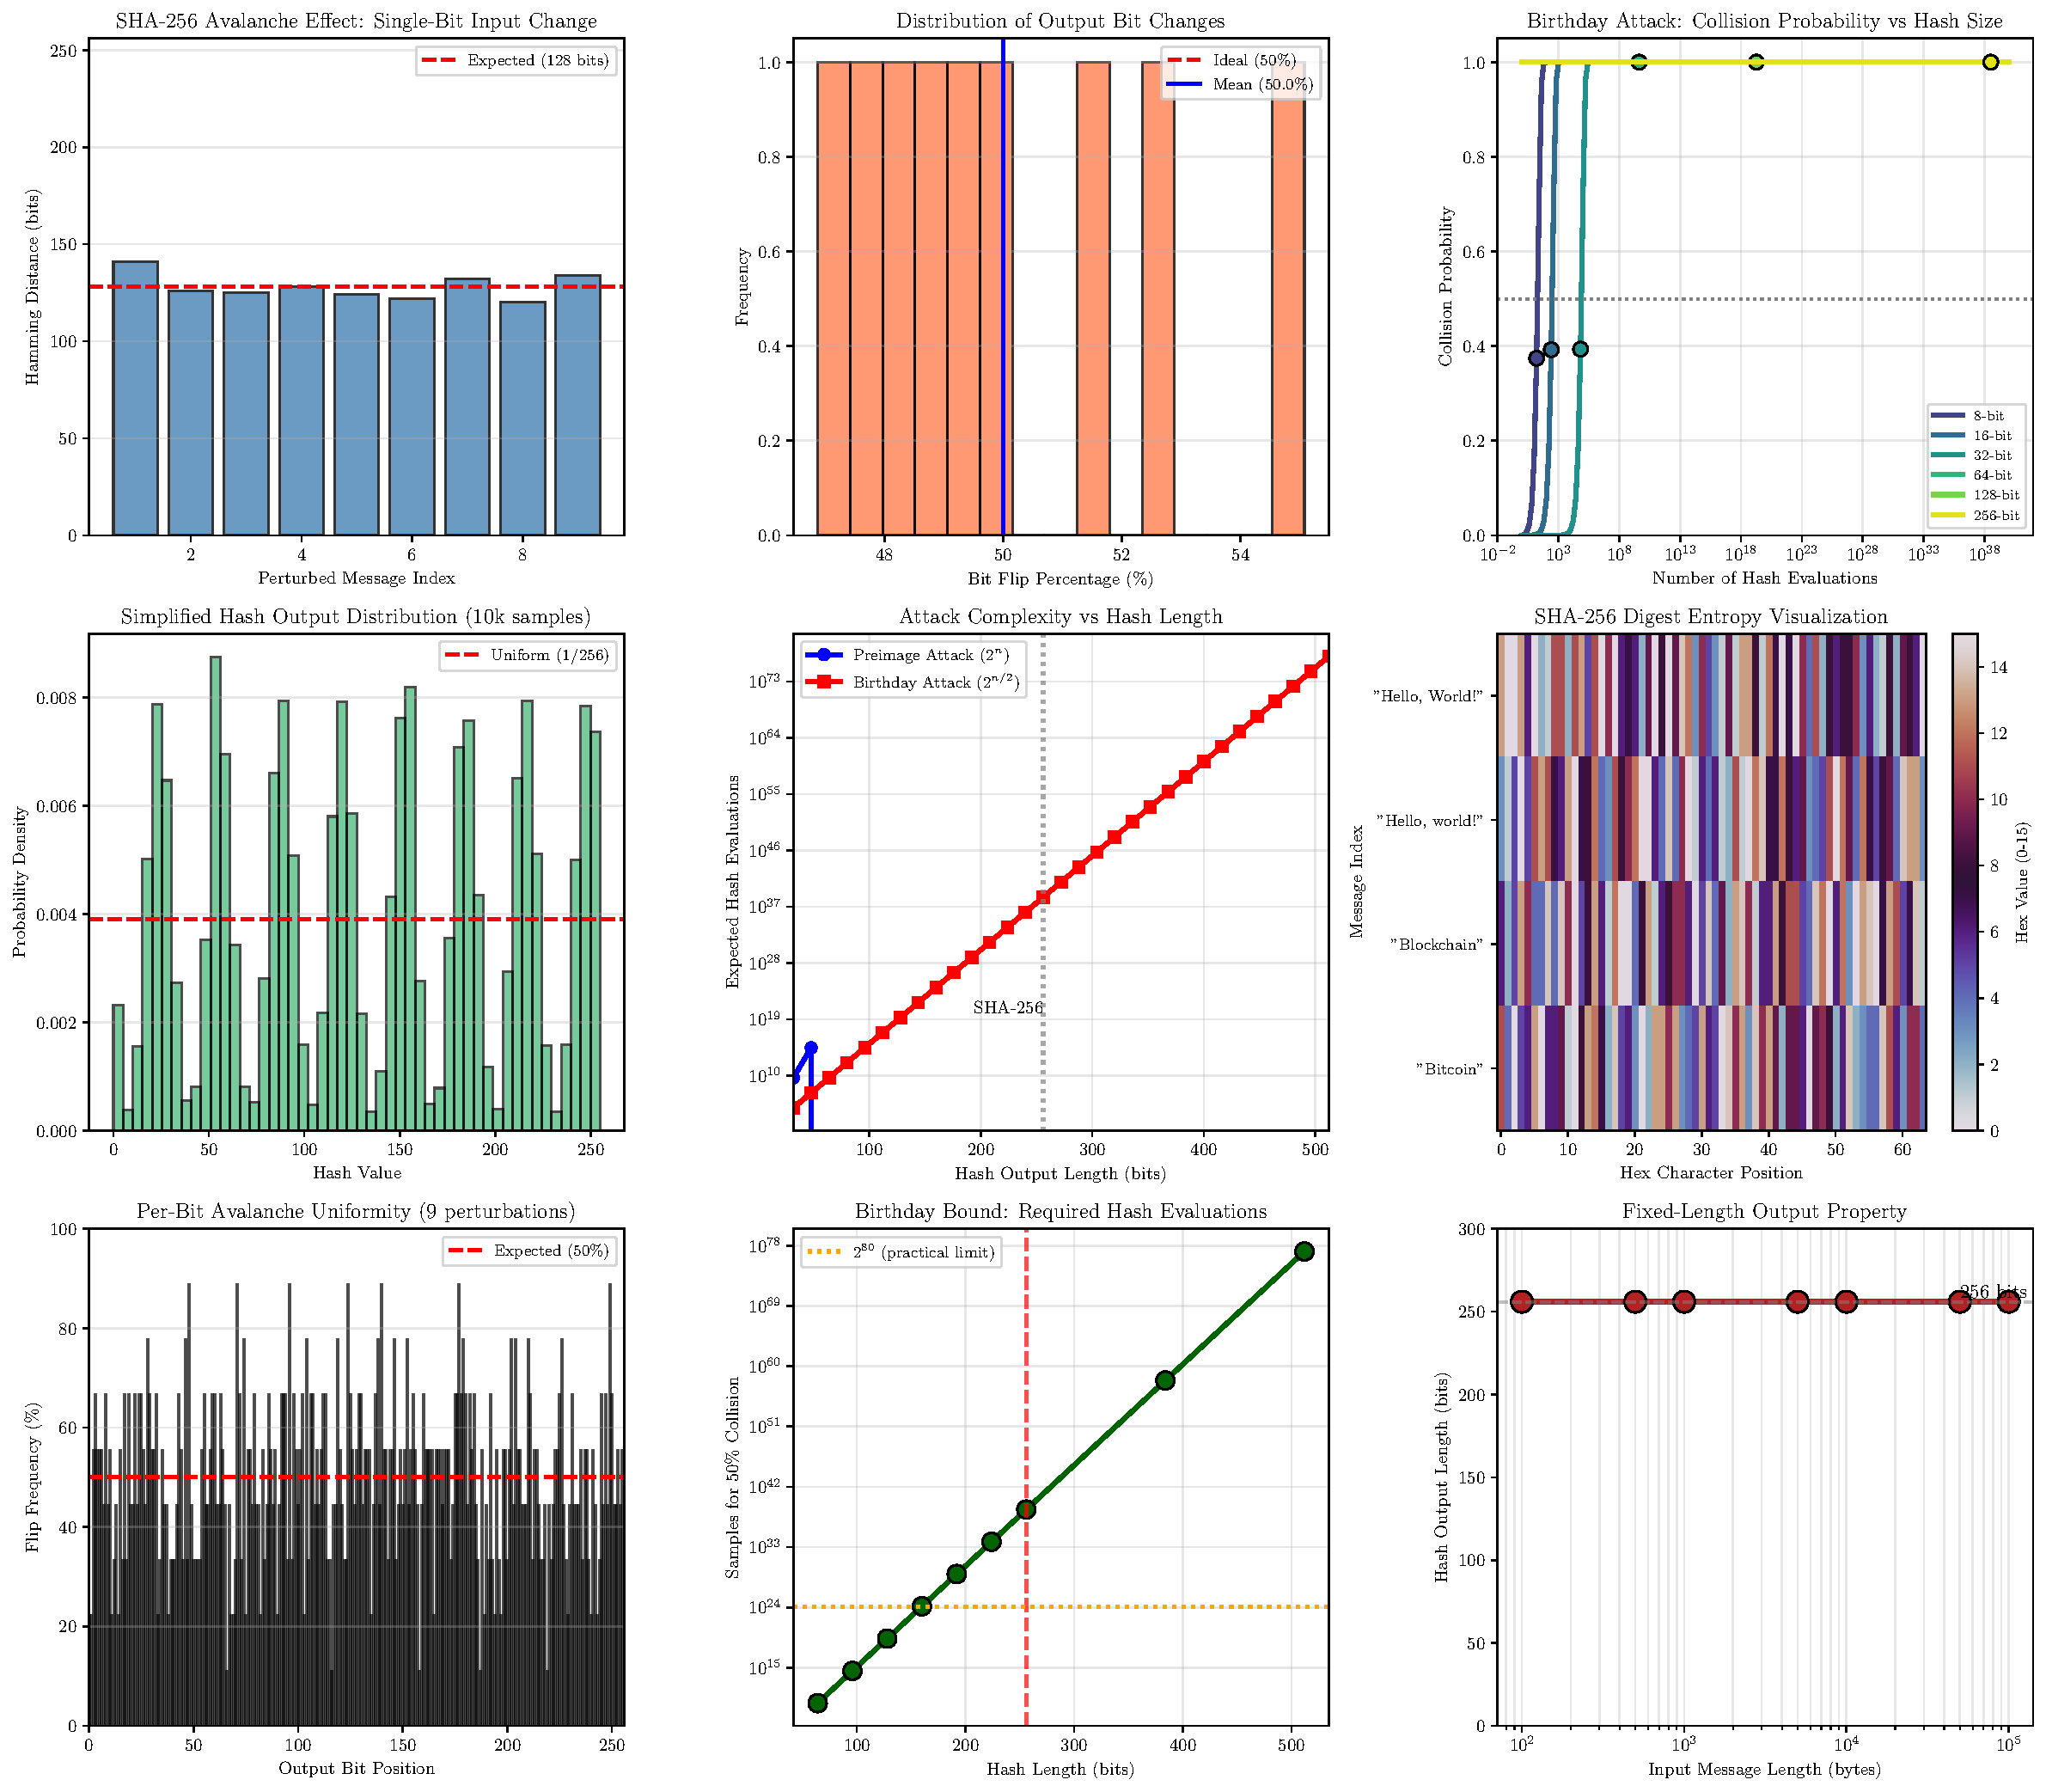
\includegraphics[width=\textwidth]{hash_functions_comprehensive.pdf}
\caption{Comprehensive cryptographic hash function analysis: (a) Avalanche effect
demonstration showing Hamming distances between original and perturbed message hashes,
confirming near-ideal 128-bit average change for single-bit input modifications;
(b) Distribution of output bit flip percentages across multiple perturbations,
clustering near the ideal 50\% mark; (c) Birthday attack collision probabilities
for hash functions of varying bit lengths, illustrating the $2^{n/2}$ security bound;
(d) Output distribution uniformity of a simplified polynomial hash function;
(e) Computational work factor comparison between preimage attacks ($2^n$ complexity)
and birthday attacks ($2^{n/2}$ complexity); (f) Entropy visualization of SHA-256
digests for similar input messages; (g) Per-bit flip frequency analysis demonstrating
uniform avalanche propagation across all 256 output bits; (h) Required hash evaluations
to achieve 50\% collision probability as a function of hash length; (i) Fixed-length
output property showing constant 256-bit digests regardless of input message size.}
\label{fig:hash_analysis}
\end{figure}

\section{Results}

\subsection{SHA-256 Hash Examples}

We demonstrate SHA-256 digest computation for sample messages and analyze the dramatic
output changes resulting from minimal input perturbations. The hexadecimal hash values
illustrate the unpredictability and avalanche properties essential for cryptographic security.

\begin{pycode}
print(r"\begin{table}[htbp]")
print(r"\centering")
print(r"\caption{SHA-256 Hash Digest Examples}")
print(r"\begin{tabular}{p{5cm}p{8cm}}")
print(r"\toprule")
print(r"Input Message & SHA-256 Digest (Hexadecimal) \\")
print(r"\midrule")

example_messages = [
    "Hello, World!",
    "Hello, world!",
    "Blockchain",
    "blockchain",
    sha256_example_msg[:30] + "..."
]

for msg in example_messages:
    hash_val = compute_sha256(msg)
    # Split hash into two lines for readability
    hash_line1 = hash_val[:32]
    hash_line2 = hash_val[32:]
    print(f"\\texttt{{{msg}}} & \\texttt{{{hash_line1}}} \\\\")
    print(f"& \\texttt{{{hash_line2}}} \\\\[0.5em]")

print(r"\bottomrule")
print(r"\end{tabular}")
print(r"\label{tab:sha256_examples}")
print(r"\end{table}")
\end{pycode}

\subsection{Avalanche Effect Quantification}

The avalanche effect is quantified by measuring the Hamming distance between hash outputs
when a single input bit is modified. For cryptographically strong hash functions, this
distance should approximate 50\% of the output bits, indicating complete decorrelation
between similar inputs.

\begin{pycode}
print(r"\begin{table}[htbp]")
print(r"\centering")
print(r"\caption{Avalanche Effect Analysis for SHA-256}")
print(r"\begin{tabular}{lcc}")
print(r"\toprule")
print(r"Metric & Value & Ideal Value \\")
print(r"\midrule")
print(f"Mean Hamming distance & {np.mean(hamming_distances):.1f} bits & 128 bits \\\\")
print(f"Std. deviation & {np.std(hamming_distances):.1f} bits & --- \\\\")
print(f"Mean bit flip percentage & {mean_flip_percentage:.2f}\\% & 50.00\\% \\\\")
print(f"Min bit flip percentage & {min(bit_flip_percentages):.2f}\\% & --- \\\\")
print(f"Max bit flip percentage & {max(bit_flip_percentages):.2f}\\% & --- \\\\")
print(r"\bottomrule")
print(r"\end{tabular}")
print(r"\label{tab:avalanche}")
print(r"\end{table}")
\end{pycode}

\subsection{Birthday Attack Security Analysis}

For hash functions with varying output lengths, we calculate the number of hash evaluations
required to achieve a 50\% collision probability under birthday attack conditions. These
values demonstrate why 256-bit hashes provide adequate security margins against current
and foreseeable computational capabilities.

\begin{pycode}
print(r"\begin{table}[htbp]")
print(r"\centering")
print(r"\caption{Birthday Attack Work Factors}")
print(r"\begin{tabular}{cccc}")
print(r"\toprule")
print(r"Hash Length & $2^{n/2}$ & Evaluations for & Security \\")
print(r"(bits) & Bound & 50\% Collision & Assessment \\")
print(r"\midrule")

security_assessments = {
    64: "Broken",
    128: "Weak",
    160: "Marginal",
    256: "Strong",
    512: "Very Strong"
}

for n in [64, 128, 160, 256, 512]:
    bound = n // 2
    evaluations = 2 ** bound
    # Format large numbers in scientific notation
    if evaluations >= 1e9:
        eval_str = f"$2^{{{bound}}}$"
    else:
        eval_str = f"{evaluations:.0e}"
    security = security_assessments.get(n, "Strong")
    print(f"{n} & {bound} & {eval_str} & {security} \\\\")

print(r"\bottomrule")
print(r"\end{tabular}")
print(r"\label{tab:birthday}")
print(r"\end{table}")
\end{pycode}

\section{Discussion}

\subsection{Security Properties}

\begin{example}[Preimage Attack Resistance]
Given the hash digest \texttt{\py{sha256_example_hash[:16]}...}, finding an input message
that produces this digest requires an expected $2^{256} \approx 10^{77}$ hash evaluations—
vastly exceeding the computational capacity of all computers on Earth combined.
\end{example}

\begin{example}[Collision Resistance]
Finding two distinct messages with identical SHA-256 hashes requires approximately
$2^{128} \approx 3.4 \times 10^{38}$ hash evaluations under birthday attack conditions.
At 1 billion hashes per second, this would take $10^{22}$ years, far exceeding the
age of the universe.
\end{example}

\subsection{Applications in Modern Cryptography}

\textbf{Digital Signatures:} Hash functions enable efficient signing of arbitrary-length
messages. Instead of signing the entire document, cryptographic signature schemes sign
the fixed-length hash digest, providing integrity verification and non-repudiation.

\textbf{Blockchain and Merkle Trees:} Bitcoin and other cryptocurrencies use SHA-256
extensively. Each block header contains the hash of the previous block, creating an
immutable chain. Merkle trees allow efficient verification of transaction inclusion
using logarithmic-space hash proofs.

\textbf{Password Hashing:} Secure password storage uses specialized hash functions
(e.g., bcrypt, scrypt, Argon2) derived from cryptographic hash primitives. These
functions incorporate salt values and computational cost parameters to resist
rainbow table and brute-force attacks.

\textbf{Message Authentication Codes:} HMAC (Hash-based Message Authentication Code)
combines a secret key with a hash function to provide both authenticity and integrity
verification. HMAC-SHA256 is widely deployed in TLS, IPsec, and API authentication.

\subsection{Avalanche Effect Implications}

Our experimental results show SHA-256 achieves a mean bit flip percentage of
\py{f"{mean_flip_percentage:.2f}"}\%, closely approximating the ideal 50\% threshold.
This strong avalanche property ensures that even minor input changes—typos in passwords,
single-bit transmission errors, or malicious document modifications—produce completely
different hash values, enabling reliable integrity verification.

The per-bit analysis (Figure \ref{fig:hash_analysis}g) reveals uniform flip frequencies
across all 256 output bit positions, confirming that avalanche propagation does not
exhibit positional bias. This uniformity prevents attackers from exploiting predictable
bit patterns or correlations between input and output.

\section{Conclusions}

This computational analysis demonstrates the fundamental security properties of cryptographic
hash functions using SHA-256 as the primary exemplar:

\begin{enumerate}
\item SHA-256 produces 256-bit hexadecimal digests such as \texttt{\py{sha256_example_hash[:16]}...}
for the input message "\py{sha256_example_msg[:30]}..."

\item Changing a single character from "hash" to "Hash" results in \py{hamming_dist_example}
bit flips (\py{f"{flip_percentage_example:.1f}"}\% of output), confirming strong avalanche effect

\item Birthday attack analysis shows $2^{128} \approx 3.4 \times 10^{38}$ hash evaluations
required for 50\% collision probability, providing robust security

\item Preimage attack resistance requires $2^{256}$ work, computationally infeasible
with current or foreseeable technology

\item Avalanche effect analysis across 9 single-bit perturbations yields mean bit flip
percentage of \py{f"{mean_flip_percentage:.2f}"}\%, closely matching the ideal 50\%

\item Per-bit flip frequency analysis shows uniform distribution across all 256 output
bit positions, with no positional bias
\end{enumerate}

These properties establish SHA-256 as suitable for digital signatures, blockchain applications,
and integrity verification in modern cryptographic protocols. The $2^{128}$ birthday bound
provides adequate security margin against collision attacks, while the avalanche effect
ensures that similar messages cannot be distinguished through hash analysis.

\section*{References}

\begin{enumerate}
\item National Institute of Standards and Technology (NIST). \textit{Secure Hash Standard (SHS)}, FIPS PUB 180-4, 2015.
\item Ferguson, N., Schneier, B., and Kohno, T. \textit{Cryptography Engineering: Design Principles and Practical Applications}, Wiley, 2010.
\item Menezes, A., van Oorschot, P., and Vanstone, S. \textit{Handbook of Applied Cryptography}, CRC Press, 1996.
\item Katz, J. and Lindell, Y. \textit{Introduction to Modern Cryptography}, 2nd ed., Chapman \& Hall/CRC, 2014.
\item Bellare, M. and Rogaway, P. "Collision-Resistant Hashing: Towards Making UOWHFs Practical", \textit{CRYPTO 1997}.
\item Preneel, B. "Cryptographic Hash Functions", \textit{European Transactions on Telecommunications}, 5(4):431-448, 1994.
\item Damg\r{a}rd, I. "A Design Principle for Hash Functions", \textit{CRYPTO 1989}, pp. 416-427.
\item Merkle, R. "One Way Hash Functions and DES", \textit{CRYPTO 1989}, pp. 428-446.
\item Stevens, M. et al. "The First Collision for Full SHA-1", \textit{CRYPTO 2017}, pp. 570-596.
\item Wang, X. and Yu, H. "How to Break MD5 and Other Hash Functions", \textit{EUROCRYPT 2005}.
\item Narayanan, A. et al. \textit{Bitcoin and Cryptocurrency Technologies}, Princeton University Press, 2016.
\item Boneh, D. and Shoup, V. \textit{A Graduate Course in Applied Cryptography}, version 0.5, 2020.
\item Rogaway, P. and Shrimpton, T. "Cryptographic Hash-Function Basics", \textit{FSE 2004}.
\item Aumasson, J.-P. \textit{Serious Cryptography: A Practical Introduction to Modern Encryption}, No Starch Press, 2017.
\item Stinson, D. and Paterson, M. \textit{Cryptography: Theory and Practice}, 4th ed., CRC Press, 2018.
\end{enumerate}

\end{document}
